% ********** Rozdział 4 **********
\chapter{Prezentacja warstwy użytkowej projektu}

Projekt "Music Player" został zaprojektowany z myślą o zapewnieniu intuicyjnego, łatwego w obsłudze i estetycznie przyjemnego interfejsu użytkownika. W tej części dokumentacji szczegółowo omówimy poszczególne komponenty interfejsu, w tym layout, nawigację, funkcje dostępne dla użytkownika oraz ogólną koncepcję i filozofię stojącą za projektowaniem UI/UX. 


\begin{figure}[!ht]
	\begin{center}
	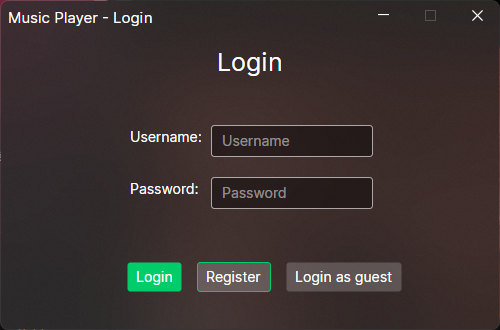
\includegraphics[height=200pt]{figures/login.png}
        \caption{{\footnotesize Formularz logowania}}
	\end{center}
\end{figure}

{Formularz logowania w aplikacji "Music Player" stanowi pierwszy punkt interakcji użytkownika z aplikacją, łącząc w sobie elegancję i prostotę. 
Tło formularza jest częściowo przezroczyste dzięki zastosowaniu efektu rozmycia, co sprawia, że prezentuje się ono za każdym razem inaczej, w zależności od tła znajdującego się pod naszą aplikacją. Pola "Username" i "Password" są intuicyjnie umieszczone w centralnym punkcie okna, co pozwala na szybkie i wygodne wprowadzenie danych przez użytkownika. Trzy przyciski akcji – "Login", "Register" oraz "Login as guest" – są wyraźnie oznaczone i zróżnicowane kolorystycznie, co nie tylko dodaje dynamiki wizualnej, ale także prowadzi użytkownika przez proces logowania krok po kroku.
}
\newpage

\begin{figure}[!ht]
	\begin{center}
	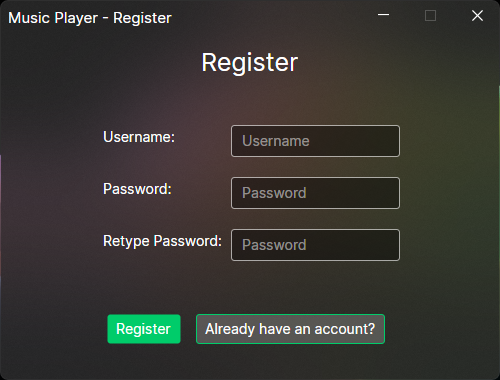
\includegraphics[height=240pt]{figures/register.png}
        \caption{{\footnotesize Formularz rejestracji}}
	\end{center}
\end{figure}

{Ekran rejestracji w aplikacji ma podobną konstrukcję do wcześniej wspomnianego ekranu logowania. Składa się z trzech głównych pól: 'Username', 'Password' oraz 'Retype Password', które są wyraźnie oznaczone i logicznie rozmieszczone, ułatwiając w ten sposób proces zakładania nowego konta. }

\begin{figure}[!ht]
	\begin{center}
	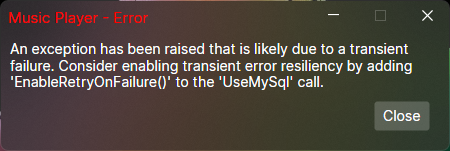
\includegraphics[]{figures/error_box.png}
        \caption{{\footnotesize Okno błędów}}
	\end{center}
\end{figure}

{
Okno błędu w aplikacji "Music Player" zostało zaprojektowane w celu przekazania ważnych informacji w sposób jasny i zwięzły. Treść okna błędu informuje o wyjątku, który został zgłoszony z powodu chwilowego problemu i sugeruje rozwiązanie techniczne, które może pomóc w jego rozwiązaniu.
Przycisk "Close" znajdujący się na dole okna jest wyraźnie zaznaczony i pozwala użytkownikowi szybko zamknąć komunikat błędu. Całość prezentuje się profesjonalnie i ma na celu ułatwienie szybkiego zidentyfikowania i rozwiązania problemu.
}

\newpage

\begin{figure}[h!]
  \centering
  \begin{minipage}{.53\textwidth}
    \centering
    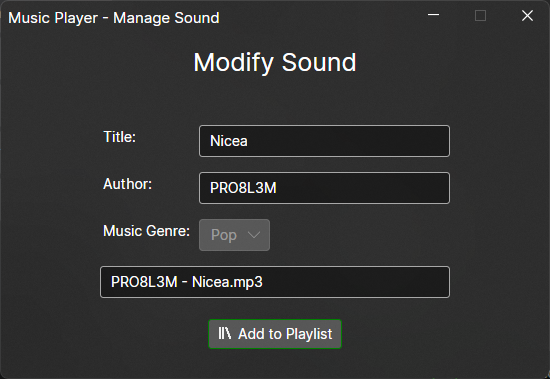
\includegraphics[width=.9\linewidth]{figures/modify1.png}
    \caption{{\footnotesize Okno edycji utworu - okno użytkownika}}
  \end{minipage}%
  \begin{minipage}{.55\textwidth}
    \centering
    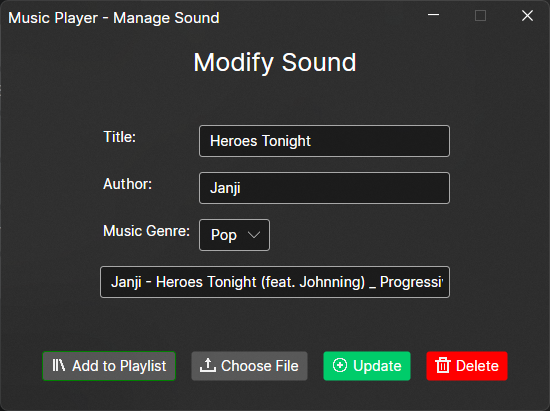
\includegraphics[width=.9\linewidth]{figures/modify2.png}
    \caption{{\footnotesize Okno edycji utowru - okno właściciela}}
  \end{minipage}
\end{figure}

{
Okna "Modify Sound" w aplikacji "Music Player" przedstawiają interfejs użytkownika umożliwiający zarządzanie informacjami o piosenkach. Są one dostosowane do różnych poziomów dostępu użytkownika, w zależności od tego, czy użytkownik dodał daną piosenkę do aplikacji.

Pierwsze okno jest przeznaczone dla użytkownika, który nie ma możliwości edycji informacji o piosence, ponieważ nie jest jej właścicielem. Prezentuje podstawowe informacje takie jak tytuł utworu ("Nicea"), autora ("PRO8L3M") oraz gatunek muzyczny ("Pop"). Na dole okna znajduje się przycisk "Add to Playlist", który pozwala na dodanie utworu do osobistej playlisty. Całość prezentuje się czysto i profesjonalnie, z zachowaniem spójnej kolorystyki i stylu.

Drugie okno jest dostępne dla użytkownika, który jest właścicielem piosenki i dlatego ma możliwość jej edycji. Użytkownik może zmieniać tytuł ("Heroes Tonight"), autora ("Janji") oraz gatunek muzyczny z dostępnego menu rozwijanego. W tym oknie dodane są dodatkowe opcje: przycisk "Choose File" umożliwia zmianę pliku muzycznego, "Update" służy do zapisania zmian, a "Delete" pozwala na usunięcie utworu z bazy danych aplikacji. Dodatkowo, utwór można dodać do playlisty za pomocą przycisku "Add to Playlist". Przyciski akcji są intuicyjnie zaprojektowane z użyciem symboli i kolorów, gdzie zielony symbolizuje akcję aktualizacji, a czerwony - usunięcie.

Oba okna są zaprojektowane z myślą o przejrzystości i łatwości użytkowania, przy jednoczesnym zachowaniu funkcjonalności i estetycznego wyglądu zgodnego z ogólnym motywem aplikacji.
}
\newpage

\begin{figure}[h!]
  \centering
  \begin{minipage}{.53\textwidth}
    \centering
    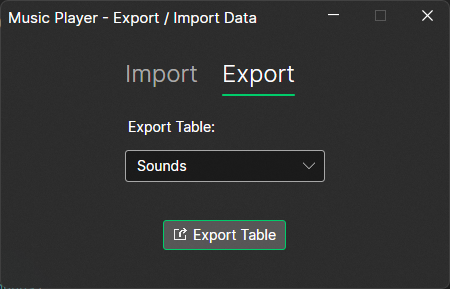
\includegraphics[width=.9\linewidth]{figures/export.png}
    \caption{{\footnotesize Okno eksportu danych}}
  \end{minipage}%
  \begin{minipage}{.55\textwidth}
    \centering
    
\includegraphics[width=.9\linewidth]{figures/import.png}
    \caption{{\footnotesize Okno importu danych}}
  \end{minipage}
\end{figure}

{
Okna importu i eksportu danych aplikacji "Music Player" są przejrzyste i funkcjonalne, umożliwiając użytkownikom łatwą migrację ich danych w formacie CSV, co jest standardem dla list utworów, playlist i informacji o użytkownikach.


\textbf{Okno eksportu danych:}
W oknie eksportu użytkownik ma możliwość wyeksportowania wybranej tabeli danych do pliku CSV. Proces jest prosty i intuicyjny – wystarczy wybrać interesującą tabelę z rozwijanego menu (np. "Sounds"), a następnie kliknąć przycisk "Export Table". To wyzwoli automatyczne pobieranie pliku CSV zawierającego wszystkie dane z wybranej tabeli. Ta funkcja jest szczególnie przydatna przy tworzeniu kopii zapasowych lub przenoszeniu danych między różnymi instancjami aplikacji.

\textbf{Okno eksportu danych:}
Okno importu danych oferuje użytkownikom możliwość załadowania danych z pliku CSV do aplikacji. Użytkownik może wybrać typ danych do importu (np. "Sounds", "Users", "Playlists") z rozwijanego menu. Pod menu znajduje się przewodnik po importowaniu, który krok po kroku informuje o sposobie importowania danych z różnych tabel. Aby zaimportować dane, użytkownik musi najpierw wybrać odpowiedni plik CSV z dysku, używając przycisku "Choose File", a następnie inicjować import przez kliknięcie "Import Table". Jest to krytyczna funkcja dla użytkowników, którzy chcą przywrócić dane lub zintegrować nowe kolekcje do swojej biblioteki.
}

\newpage

\begin{figure}[!ht]
	\begin{center}
	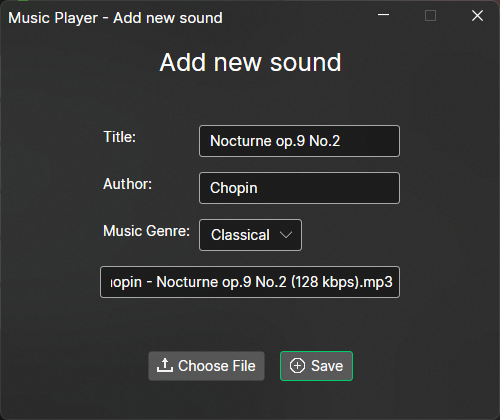
\includegraphics[]{figures/add_new_sound.png}
        \caption{{\footnotesize Formularz dodawania utworów}}
	\end{center}
\end{figure}

{Okno "Add new sound" w aplikacji "Music Player" jest przeznaczone do łatwego dodawania nowych utworów do biblioteki użytkownika. Użytkownicy mogą wprowadzić metadane dla każdego nowego dźwięku, takie jak tytuł utworu, autora oraz gatunek muzyczny z rozwijanego menu, gdzie można wybrać np. Classical, Pop, Rock, Jazz. Te pola pozwolą na lepszą organizację i wyszukiwanie w przyszłości.

Pole na dole, gdzie wyświetlana jest nazwa pliku, pokazuje wybrany utwór do dodania, który użytkownik załadował przez przycisk "Choose File". Po wybraniu pliku, utwór może być dodany do biblioteki aplikacji za pomocą przycisku "Save", który jest wyraźnie widoczny i łatwy do zlokalizowania.
Proces dodawania jest intuicyjny i zaprojektowany tak, aby maksymalnie uproszczać zarządzanie kolekcją muzyki użytkownika.}

\newpage

\begin{figure}[!ht]
	\begin{center}
	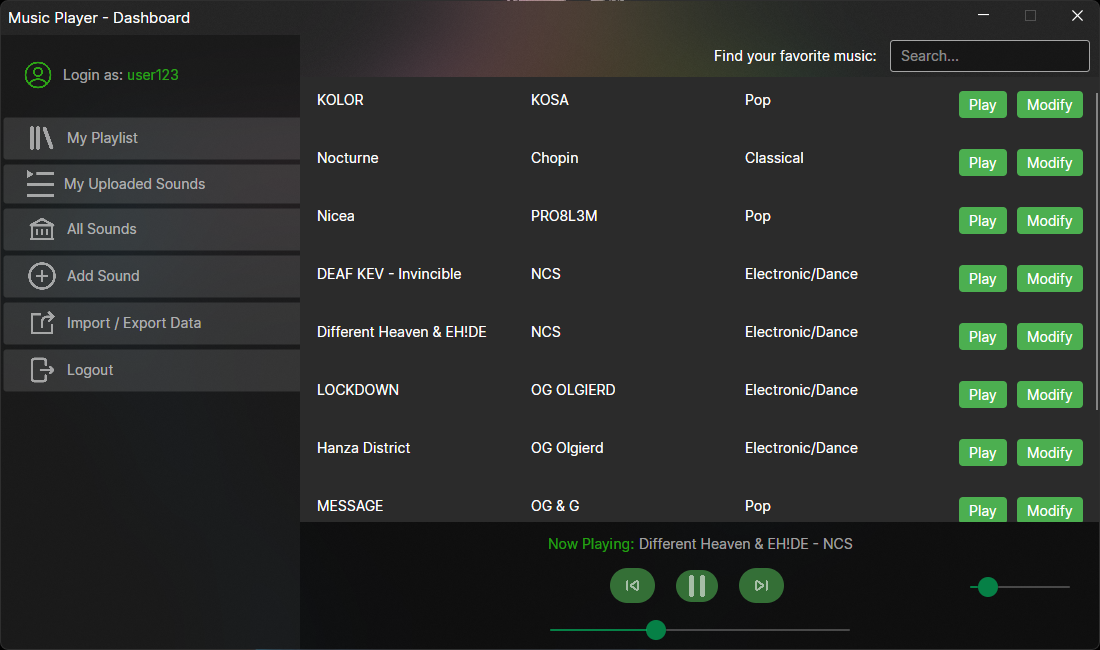
\includegraphics[width=500pt]{figures/main1.png}
        \caption{{\footnotesize Główne okno aplikacji}}
	\end{center}
\end{figure}

{
Główne okno aplikacji "Music Player" to centrum dowodzenia dla użytkownika, gdzie może zarządzać swoją muzyczną biblioteką i odtwarzaniem. Na lewym pasku bocznym znajduje się intuicyjne menu nawigacyjne z ikonami, które umożliwiają szybki dostęp do różnych sekcji aplikacji, takich jak "My Playlist", "My Uploaded Sounds", "All Sounds", a także opcje do dodawania nowych dźwięków i importu/eksportu danych. Na dole znajduje się opcja "Logout", która pozwala użytkownikowi bezpiecznie wylogować się z aplikacji.

W centralnej części okna znajduje się lista utworów z ich tytułami, autorami i gatunkami muzycznymi. Każdy wpis na liście ma przypisane przyciski "Play" i "Modify", które pozwalają odpowiednio na odtwarzanie wybranego utworu oraz jego edycję – ta druga opcja jest dostępna tylko dla utworów dodanych przez zalogowanego użytkownika.

Na górze tego panelu znajduje się pasek wyszukiwania, który umożliwia szybkie znalezienie ulubionej muzyki według nazwy utworu, wykonawcy lub gatunku.

Dolna część ekranu to dedykowany pasek odtwarzacza z podstawowymi przyciskami sterowania odtwarzaniem (play, pause, skip), a także pasek postępu, który wizualnie pokazuje postęp aktualnie odtwarzanego utworu. Ponadto wyświetlana jest nazwa aktualnie odtwarzanego utworu, co pozwala użytkownikowi na szybką identyfikację odtwarzanej kompozycji.

Całość interfejsu utrzymana jest w ciemnej kolorystyce, co jest przyjemne dla oka i nie męczy wzroku podczas dłuższego korzystania z aplikacji w różnych warunkach oświetleniowych.

}

\newpage

\begin{figure}[!ht]
	\begin{center}
	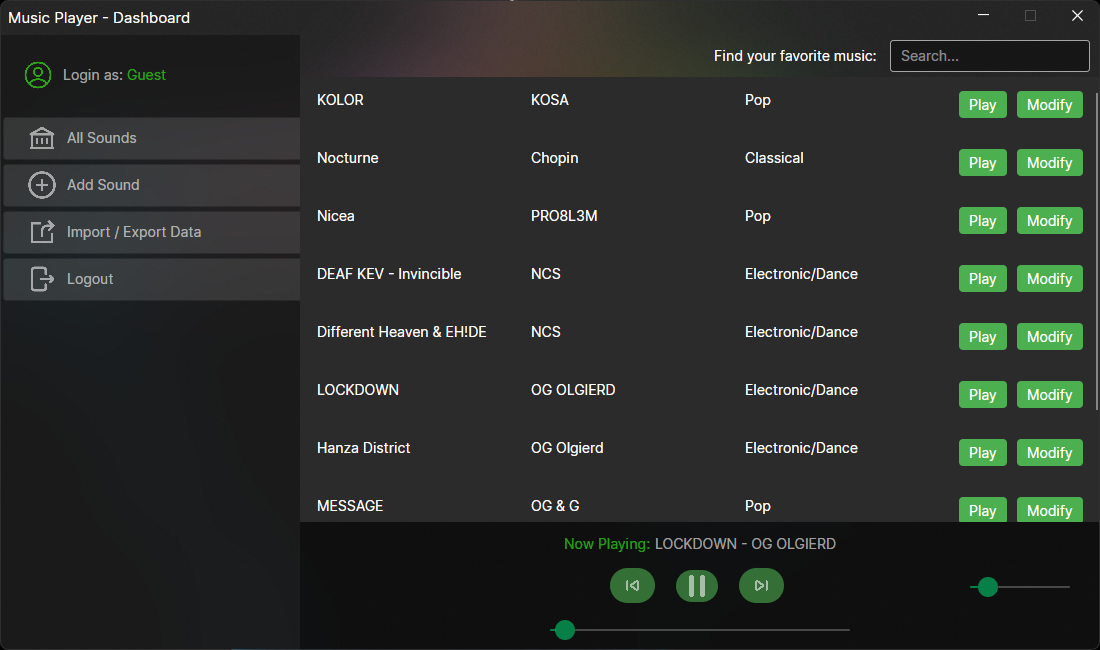
\includegraphics[width=500pt]{figures/main_guest.png}
        \caption{{\footnotesize Główne okno aplikacji - widok gościa}}
	\end{center}
\end{figure}

{W porównaniu do wcześniejszego okna dashboardu dla zalogowanego użytkownika, obecne okno dla gościa prezentuje się bardzo podobnie, z tą różnicą, że nie zawiera opcji "My Playlist" ani "My Uploaded Sounds". To wskazuje na ograniczoną funkcjonalność dostępną dla użytkowników, którzy nie są zalogowani lub korzystają z aplikacji jako goście.

Status logowania na górze okna zmienia się z konkretnego identyfikatora użytkownika (np. user123) na ogólne oznaczenie "Guest", co podkreśla, że użytkownik nie jest obecnie zalogowany i korzysta z aplikacji w ograniczonym zakresie. Użytkownik gość ma dostęp do ogólnej listy utworów w sekcji "All Sounds", może przeszukiwać dostępną muzykę i korzystać z funkcji odtwarzania, ale nie posiada możliwości modyfikacji listy utworów ani zarządzania własnymi dźwiękami. Może również wyeksportować/importować dane i wylogować się z systemu, co wskazuje na pewne podstawowe interakcje, które są dostępne dla każdego, kto korzysta z aplikacji.}

% ********** Koniec rozdziału **********
